\subsection{Plots erzeugen}
Aus den oben gelesenen Daten kann nun ein Plot erzeugt werden. 

Zuerst mal ein ganz einfacher Plot.

\randnotiz{Plot erzeugen}\lstinputlisting[language=Python]{chapters/advancedTopics/src/machinelearning/plot.py}\label{defineplot1:lst:plot}

Die erzeugt den Plot wie in ~\ref{ml:samples:ml_sample_plot} dargestellt.

\begin{figure}[ht]
	\centering
	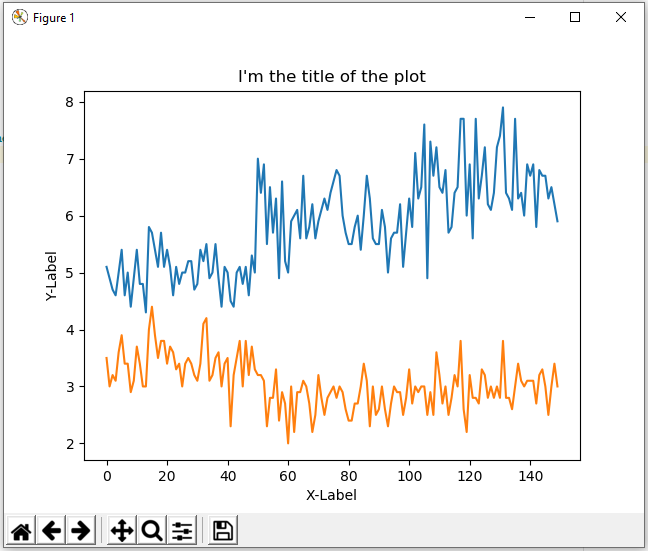
\includegraphics[width=1\textwidth]{images/MachineLearning/ml_sample_plot.png}
	\caption{Plot mit Titel und Achsenbeschriftungen}
	\label{ml:samples:ml_sample_plot}
\end{figure}


Eine weitere Darstellungsform k�nnte als Histogramm sein.

\randnotiz{Histogramm erzeugen}\lstinputlisting[language=Python]{chapters/advancedTopics/src/machinelearning/plothist.py}\label{defineplot1:lst:plothist}

Das erzeugte Histogramm sieht aus wie in Abbildung ~\ref{ml:samples:ml_sample_plothist}.

\begin{figure}[ht]
	\centering
	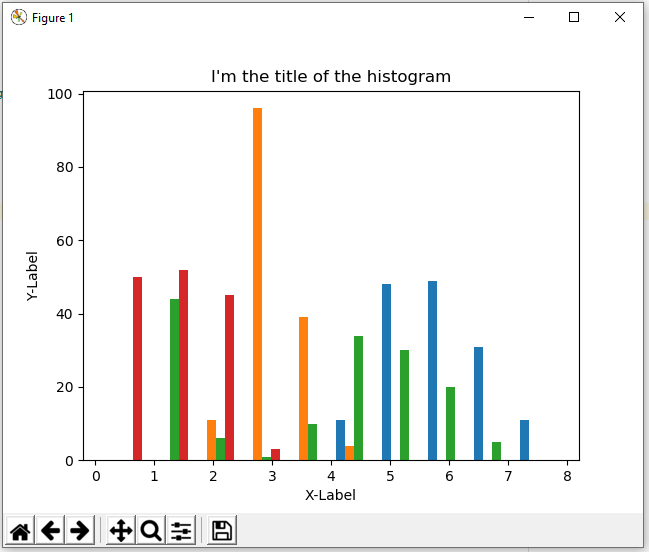
\includegraphics[width=1\textwidth]{images/MachineLearning/ml_sample_plothist.png}
	\caption{Histogram-Plot mit Titel und Achsenbeschriftungen}
	\label{ml:samples:ml_sample_plothist}
\end{figure}

F�r das Beispiel oben bietet sich au�erdem die Darstellung in einem Scatterplot an.

\randnotiz{Scatterplot erzeugen}\lstinputlisting[language=Python]{chapters/advancedTopics/src/machinelearning/plotscatter.py}\label{defineplot1:lst:plotscatter}

Der Code erzeugt einen Scatterplot wie in Abbildung ~\ref{ml:samples:ml_sample_plotscatter}.

\begin{figure}[ht]
	\centering
	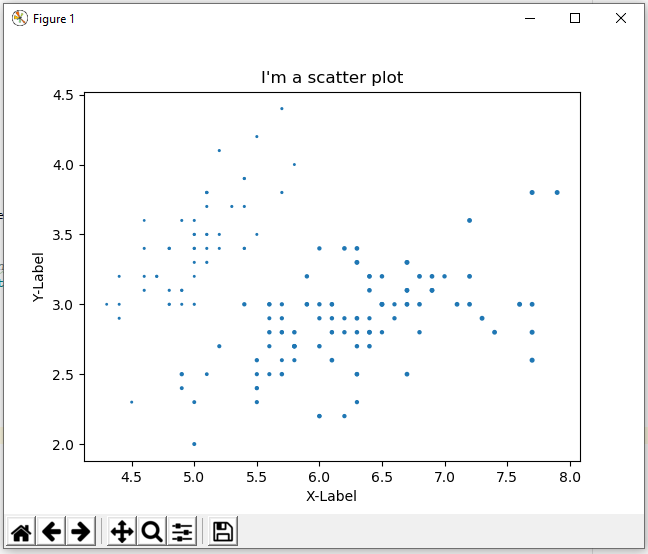
\includegraphics[width=1\textwidth]{images/MachineLearning/ml_sample_plotscatter.png}
	\caption{Scatter-Plot mit Titel und Achsenbeschriftungen}
	\label{ml:samples:ml_sample_plotscatter}
\end{figure}

\uebung
\aufgabe{MachineLearning/machinelearning_plots}